\documentclass[11pt, landscape, a4paper]{article}
\usepackage{geometry}[landscape]
\usepackage{multicol}
\usepackage{graphicx}
\usepackage{amsmath} 
\usepackage{amssymb}

\usepackage[dvipsnames]{xcolor}
\usepackage{mathptmx}
\usepackage[compact]{titlesec}
\usepackage{paralist}

\usepackage{tabularx}
\usepackage{ctable}

% Set page margins
\geometry{top=.0cm, left=.0cm, right=.0cm, bottom=.0cm}

% Set indentation
\setlength{\parindent}{0pt}
\setlength{\parskip}{0cm}

% Set path for assets
\graphicspath{{assets/}}

\setlength{\columnsep}{5pt}
\raggedcolumns

% _____ CUSTOM COMMANDS __________________________________________
\newcommand{\E}[0]{\mathbb{E}}
\newcommand{\N}[0]{\mathbb{N}}
\newcommand{\R}[0]{\mathbb{R}}

\newcommand{\sgn}[0]{\text{sgn}}

\newcommand{\argmin}[1]{\underset{#1}{\text{argmin}}}
\newcommand{\argmax}[1]{\underset{#1}{\text{argmax}}}

\titlespacing{\section}{0pt}{0.3ex}{0ex}
\titlespacing{\subsection}{0pt}{0ex}{0ex}
\linespread{0.7}

\newcommand*{\myfont}{\fontfamily{phv}\selectfont}

\titleformat*{\section}{\fontsize{11}{11}\selectfont\myfont\bfseries\color{Emerald}}
\titleformat*{\subsection}{\fontsize{11}{11}\selectfont\myfont\bfseries\color{purple}}
\begin{document}
\begin{multicols*}{4}

\setlength{\abovedisplayskip}{0pt}
\setlength{\belowdisplayskip}{0pt}
\setlength{\abovedisplayshortskip}{0pt}
\setlength{\belowdisplayshortskip}{0pt}

% _____ CONTENT __________________________________________________

% main heading
%\begin{center}
%	\Large{\te xtbf{Introduction to ML}} \\
%    \small{by dcamenisch}
%\end{center}

\section*{Model Error}

\textbf{Empirical Risk} \quad \ $\hat R_D(f) = \frac{1}{n} \sum \mathcal \ell(y, f(x))$

\textbf{Population Risk} \quad $R(f) = \E_{x,y \sim p}[\ell(y, f(x))]$

It holds that $\E_D[\hat R_D (\hat f)] \leq R(\hat f)$. We call $R(\hat f)$ the generalization error.

\textbf{Bias Variance Tradeoff}:

Pred. error = \color{red} Bias$^2$ \color{black} + \color{blue} Variance \color{black} + \color{ForestGreen} Noise \color{black}
\begin{align*}
	\E_D[R(\hat f)] &= \color{red} \E_x[f^*(x) - \E_D[\hat f_D(x)]]^2 \\[-4pt]
 	&+ \color{blue} \E_x[\E_D[(\hat f_D(x) - \E_D[\hat f_D(x)])^2]] \color{black}  + \color{ForestGreen} \sigma
\end{align*}

\textbf{Bias}: how close $\hat f$ can get to $f^*$

\textbf{Variance}: how much $\hat f$ changes with $D$

\section*{Regression}

\textbf{Squared loss} \quad (convex)

\qquad \qquad $\frac{1}{n}\sum (y_i - f(x_i))^2 = \frac{1}{n}||y - X w||_2^2$

\qquad \qquad $\nabla_w L(w) = 2X^\top(Xw -y)$

Solution: $\hat{w} = (X^\top X)^{-1}X^\top y$

\subsection*{Regularization}

\textbf{Lasso Regression} \quad (sparse)

\qquad \qquad $\argmin{w \in \R^d} ||y - \Phi w||_2^2 + \lambda ||w||_1$

\textbf{Ridge Regression}

\qquad \qquad $\argmin{w \in \R^d} ||y - \Phi w||_2^2 + \lambda ||w||_2^2$

\qquad \qquad $\nabla_w L(w) = 2X^\top(Xw -y) + 2 \lambda w$

Solution: $\hat w = (X^\top X + \lambda I)^{-1} X^\top y$

large $\lambda \Rightarrow$ larger bias but smaller variance 

\subsection*{Cross-Validation}

\begin{compactitem}
	\item For all folds $i = 1,..., k$: 
		\begin{compactitem}
			\item Train $\hat{f}_i$ on $D' - D'_i$
			\item Val. error $R_i = \frac{1}{|D'_i|} \sum \ell(\hat{f}_i(x), y)$
		\end{compactitem}
	\item Compute CV error $\frac{1}{k} \sum_{i=1}^k R_i$
	\item Pick model with lowest $CV$ error
\end{compactitem}
\section*{Gradient Descent}
Converges only for convex case.
\[
	w^{t+1} = w^t - \eta_t \cdot \nabla \ell(w^t)
\]

For linear regression:
\[
	||w^t - w^*||_2 \leq ||I - \eta X^\top X||_{op}^t ||w^0 - w^*||_2
\]

$\rho = ||I - \eta X^\top X||_{op}^t$ conv. speed for const. $\eta$. Opt. fixed $\eta = \frac{2}{\lambda_{\text{min}} + \lambda_{\text{max}}}$ and max. $\eta \leq \frac{2}{\lambda_{\text{max}}}$. 

\textbf{Momentum}: $w^{t+1} = w^t + \gamma \Delta w^{t-1} - \eta_t \nabla \ell(w^t)$
Learning rate $\eta_t$ guarantees convergence if $\sum_t \eta_t = \infty$ and $\sum_t \eta_t^2 < \infty$

\section*{Classification}

\textbf{Zero-One loss} \quad not convex or continuous

\qquad \qquad $\ell_{0-1}(\hat{f}(x), y) = \mathbb{I}_{y \neq \sgn \hat{f}(x)}$

\textbf{Logistic loss} \quad $\log(1 + e^{-y \hat{f}(x)})$

\qquad \qquad $\nabla \ell(\hat{f}(x), y) = \frac{-y_i x_i}{1 + e^{y_i \hat{f}(x)}}$

\textbf{Hinge loss} \quad \ $\max(0, 1-y \hat{f}(x))$

\textbf{Softmax} $p(1 | x) = \frac{1}{1 + e^{- \hat{f}(x)}}, p(-1 | x) = \frac{1}{1 + e^{\hat{f}(x)}}$ 

Multi-Class \ \ \ $\hat{p}_k = e^{\hat{f}_k(x)} / \sum_{i=1}^K e^{\hat{f}_j(x)}$

\subsection*{Linear Classifiers}

$f(x) = w^\top x$, the decision boundary $f(x) = 0$. \smallskip

If data is lin. sep., grad. desc. converges to \textbf{Maximum-Margin Solution}: 

\quad $w_\text{MM} = \text{argmax} \; \text{margin} (w) \; \text{with } ||w||_2 = 1$

Where $\text{margin} (w) = \min_i y_i w^\top x_i$.
 
\subsection*{Support Vector Machines i.o.i}
\textbf{Hard SVM}

\qquad $\hat{w} = \min_w ||w||_2 \; \; \text{s.t. } \forall i \;y_i w^\top x_i \geq 1$
 
\textbf{Soft SVM} \quad allow "slack" in the constraints
$$\hat{w} = \min_{w, \xi} \frac{1}{2} ||w||_2^2 + \lambda \sum_{i=1}^n \underbrace{\max (0, 1 - y_i w^\top x_i)}_{\text{hinge loss}}$$ \\[-20pt]

\subsection*{Metrics} 
Choose $+1$ as the more important class. 

\begin{multicols*}{2}
	\begin{center}
		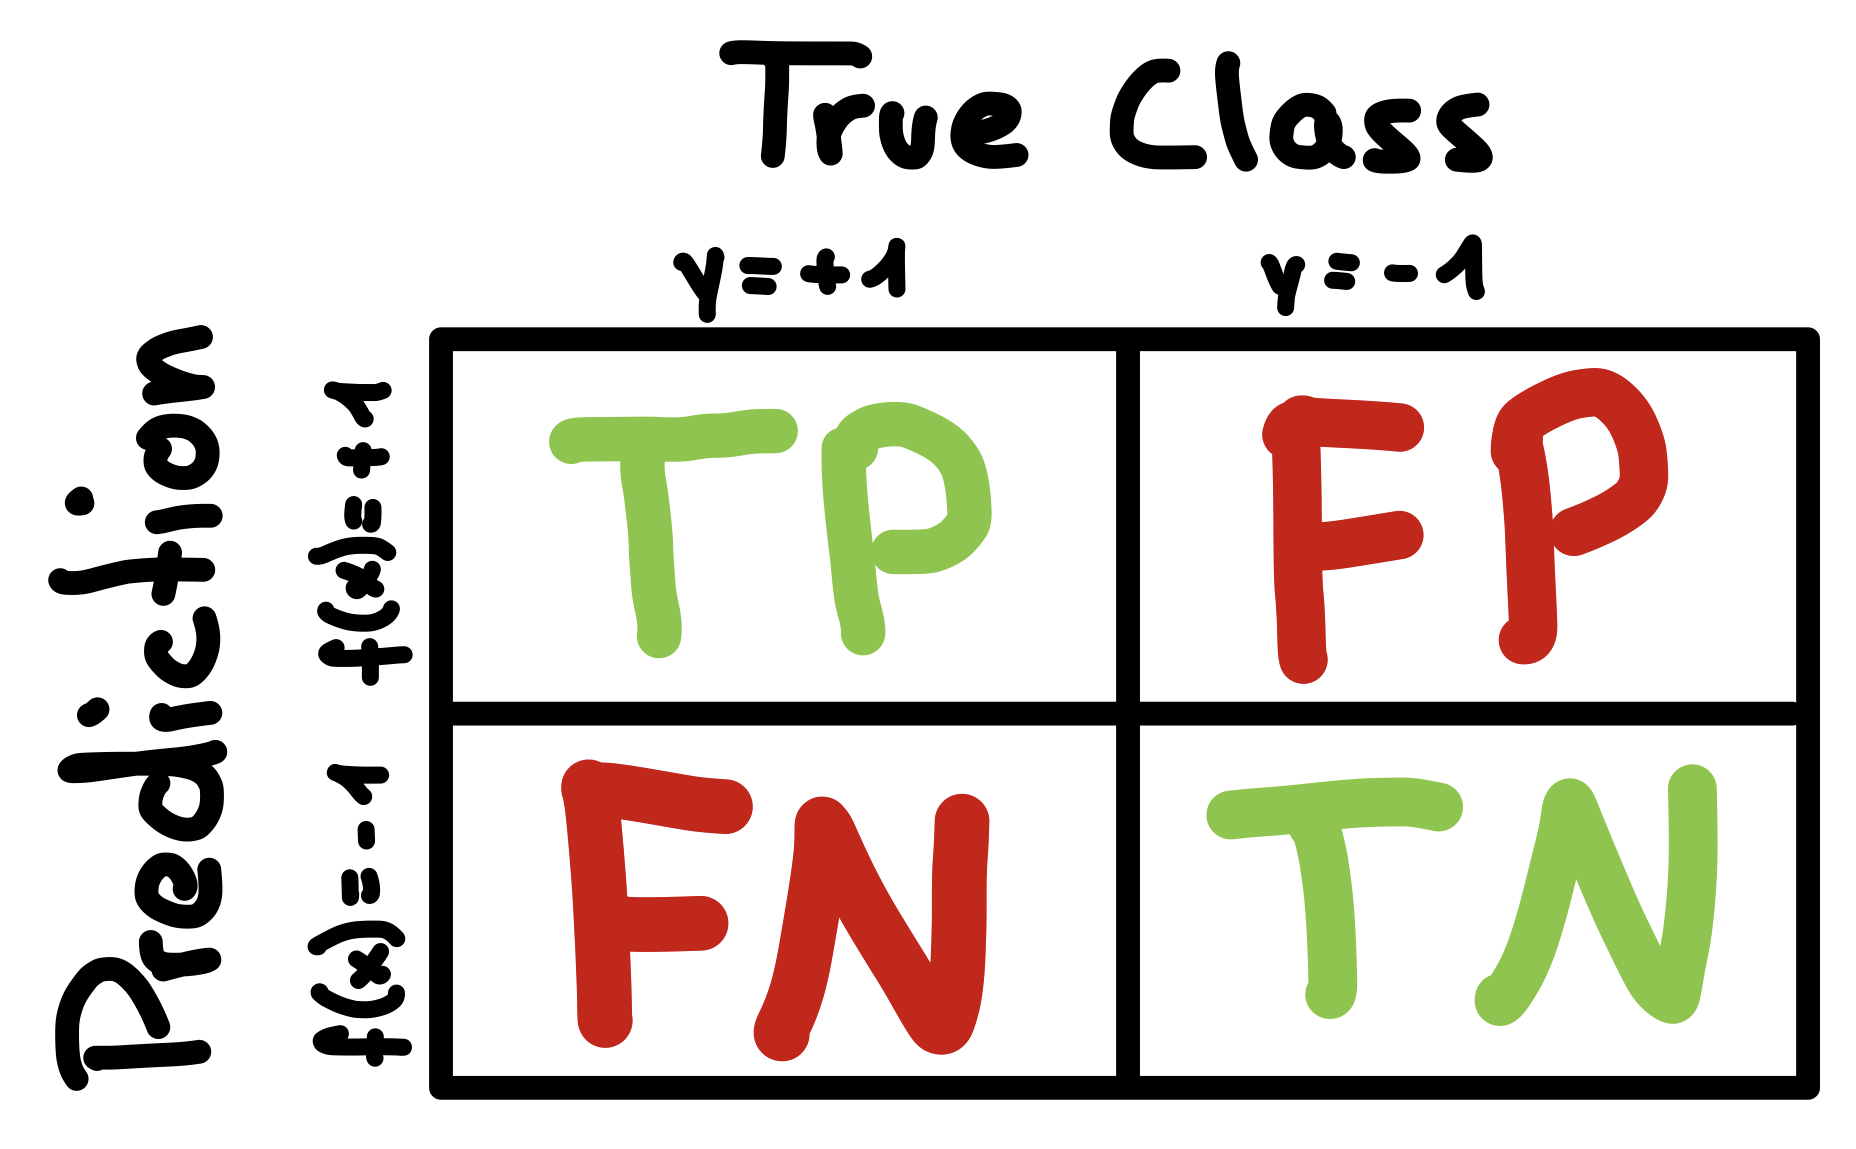
\includegraphics[width=\columnwidth]{confusion-matrix.jpeg}
	\end{center}
	
	$\text{error}_1 / \text{FPR}: \frac{\text{FP}}{\text{TN + FP}}$
	$\text{error}_2 / \text{FNR}: \frac{\text{FN}}{\text{TP + FN}}$
	$\text{Precision}: \frac{\text{TP}}{\text{TP + FP}}$
	$\text{TPR / Recall}: \frac{\text{TP}}{\text{TP + FN}}$
\end{multicols*}

.\\[-20pt]
\textbf{AUROC}: Plot TPR vs. FPR and compare different ROC's with area under the curve.

\textbf{F1-Score}: $\frac{2\text{TP}}{2\text{TP + FP + FN}}$, $\text{Accuracy}: \frac{\text{TP + TN}}{\text{P + N}}$

Goal: large recall and small FPR.
  
\section*{Kernels}

Parameterize: $w = \Phi^\top \alpha$, $K = \Phi \Phi^\top$

A kernel is \textbf{valid} if $K$ is sym.: $k(x,z) = k(z,x)$ and psd: $z^\top K z \geq 0$

\textbf{lin.}: $k(x, z) = x^\top z$, 
\textbf{rbf}: $k(x, z) = \exp ( -\frac{||x - z||_\alpha}{\tau} )$
\textbf{poly.}: $k(x, z) = (x^\top z + 1)^m$ $\mathcal{O}(n^2 * d)$

$\alpha = 1 \Rightarrow $ laplacian kernel \\
$\alpha = 2 \Rightarrow $ gaussian kernel

\textbf{Kernel composition rules}

$k = k_1 + k_2$, \quad $k = k_1 \cdot k_2$ \quad $\forall c > 0. \; k = c \cdot k_1$,
$\forall f \text{ convex}. \; k = f(k_1), $ holds for polynoms with pos. coefficients or exp function. 

$\forall f. \; k(x,y) = f(x)k_1(x,y)f(y)$

\textbf{Mercers Theorem}: Valid kernels can be decomposed into a lin. comb. of inner products.

\textbf{Kern. Ridge Reg.}
$\frac{1}{n} ||y - K\alpha ||_2^2 + \lambda \alpha^\top K \alpha$

$\mathcal{O}(d^m)$ for large d, $\mathcal{O}(m^d)$ for large  m

\section*{KNN Classification}

\begin{compactitem}
	\item Pick $k$ and distance metric $d$
	\item For given $x$, find among $x_1,...,x_n \in D$ the $k$ closest to $x \to x_{i_1},..., x_{i_k}$
	\item Output the majority vote of labels
\end{compactitem}
\section*{Neural Networks}
$w$ are the weights and $\varphi: \R \mapsto \R$ is a nonlinear \textbf{activation function}: $\phi(x, w) = \varphi(w^\top x)$


$\textbf{ReLU: } \max (0,z), \; \textbf{Tanh: } \frac{\exp(z) - \exp(-z)}{\exp(z) + \exp(-z)}$ \\[-3pt]
$\textbf{Sigmoid: } \frac{1}{1 + \exp(-z)}$


\textbf{Universal Approximation Theorem}: We can approximate any arbitrary smooth target function, with 1+ layer with sufficient width.

\subsection*{Forward Propagation}

Input: $v^{(0)} = [x; 1]$ \quad Output: $f = W^{(L)} v^{(L-1)}$
Hidden: $z^{(l)} = W^{(l)} v^{(l-1)}, v^{(l)} = [\varphi(z^{(l)}); 1]$


\subsection*{Backpropagation}

Non-convex optimization problem: \\[-10pt]

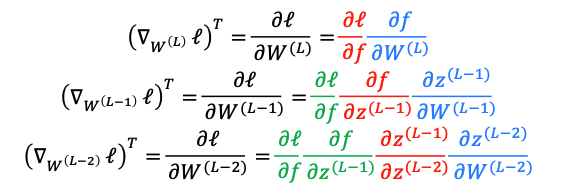
\includegraphics[width=\columnwidth]{backpropagation.png} \\[-15pt]

Only compute \color{Red} \textbf{the gradient}\color{Black}. Rand. init. weights by distr. assumption for $\varphi$. ( $2 / n_{in}$ for ReLu and $1/n_{in}$ or $ 1/ (n_{in} + n_{out})$ for Tanh)

\subsection*{Overfitting}
\textbf{Regularization}; \textbf{Early Stopping}; \textbf{Dropout}: ignore hidden units with prob. $p$, after training use all units and scale weights by $p$; \textbf{Batch Normalization}: normalize the input data (mean 0, variance 1) in each layer

\subsection*{CNN \quad \color{Black}$\varphi(W * v^{(l)})$}
For each channel there is a separate filter.

\subsection*{Convolution}
    $K = kernelSize$ $C = channel$ $F = filter$ $inputSize = I$ $padding = P$
    $stride = S$ 
\begin{align*}
    \text{Number of parameters} &= K^{dimensions} C F\\
    \text{Output size} &= \frac{I + 2P - K}{S} + 1\\
    \text{Inputs} &= W * H * D * C * N
\end{align*}


\section*{Unsupervised Learning}



\subsection*{k-Means Clustering}

Optimization Goal (non-convex):

\qquad $\hat{R} (\mu) = \sum_{i=1}^n \min_{j\in \{1,\ldots,k\}} ||x_i - \mu_j||_2^2$

Lloyd's heuristics:
Init.cluster centers $\mu^{(0)}$:
\begin{compactitem}
	\item Assign points to closest center				
	\item Update $\mu_i$ as mean of assigned points
\end{compactitem}

Converges in exponential time.

Initialize with \textbf{k-Means++}:

\begin{compactitem}
	\item Random data point $\mu_1 = x_i$
	\item Add seq $\mu_2, \ldots ,\mu_k$ rand., with prob:
		$\text{given } \mu_{1:j} \text{ pick } \mu_{j+1} = x_i$ 
		$\text{ where } p(i) = \frac{1}{z} \min_{l \in \{1,\ldots,j\}} ||x_i - \mu_l||_2^2$
\end{compactitem}
Converges expectation $\mathcal O (\log k) * \text{opt.solution}$.
Find $k$ by negligible loss decrease or reg.

\subsection*{Principal Component Analysis}

Optimization goal:
$\argmin{||w||_2 = 1, z} \sum_{i=1}^n ||x_i - z_i w||_2^2$

The optimal solution is given by $z_i = w^\top x_i$.  

Substituting gives us:

\qquad \qquad $\hat{w} = \text{argmax}_{||w||_2=1} \; w^\top \Sigma w$

Where $\Sigma = \frac{1}{n} \sum_{i=1}^n x_i x_i^\top$ is the empirical covariance. Closed form solution given by the principal eigenvector of $\Sigma$, i.e. $w = v_1$ for $\lambda_1 \geq \cdots \geq \lambda_d \geq 0$:
$\Sigma = \sum_{i=1}^d \lambda_i v_i v_i^\top$

For $k > 1$ we have to change the normalization to $W^\top W = I$ then we just take the first $k$ principal eigenvectors so that $W = [v_1, \ldots, v_k]$.

\subsection*{PCA through SVD}
\begin{compactitem}
	\item The first $k$ col of $V$ where $X = U S V^\top$.
	\item linear dimension reduction method
	\item first principal component eigenvector of data covariance matrix with largest eigenvalue
	\item covariance matrix is symmetric $\rightarrow$ all principal components are mutually orthogonal
\end{compactitem}	

\subsection*{Kernel PCA}

$\Sigma = \frac{1}{n} \sum_{i=1}^n x_i x_i^\top = X^\top X \Rightarrow$  kernel trick:

\qquad \qquad $\hat{\alpha} = \text{argmax}_\alpha \; \frac{\alpha^\top K^\top K \alpha}{\alpha^\top K \alpha}$

Closed form solution:

$\alpha^{(i)} = \frac{1}{\sqrt{\lambda_i}}v_i \quad K = \sum_{i = 1}^n \lambda_i v_i v_i^\top, \lambda_1 \geq \cdots \geq 0$

A point $x$ is projected as:
$z_i = \sum_{j=1}^n \alpha_j^{(i)} k(x_j, x)$

\subsection*{Autoencoders}

We want to minimize $\frac{1}{n}\sum_{i=1}^n ||x_i - \hat{x}_i||_2^2$.
\[
	\hat{x} = f_{dec}(f_{enc}(x, \theta_{enc}); \theta_{dec})
\]

Lin.activation func. \& square loss $=>$ PCA
\section*{Statistical Perspective}

Assume that data is generated iid. by some $p(x, y)$. We want to find $f: X \mapsto Y$ that minimizes the \textbf{population risk}.

\subsection*{Opt. Predictor for the Squared Loss}

$f$ minimizing the population risk:

\qquad $f^*(x) = \E[y \; | \; X = x] = \int y \cdot p(y \; | \; x) dy$

Estimate $\hat{p}(y \; | \; x)$ with MLE:
\begin{align*}
	\theta^* &= \argmax{\theta} \; \hat{p}(y_1, ..., y_n \; | \; x_1, ..., x_n, \theta) \\[-10pt]
	&= \argmin{\theta} \; - \sum_{i=1}^n \log p(y_i \; | \; x, \theta) 
\end{align*} \\[-11pt]

The MLE for linear regression is unbiased and has minimum variance among all unbiased estimators. However, it can overfit.

\subsection*{Ex. Conditional Linear Gaussian}

Assume Gaussian noise $y = f(x) + \epsilon$ with $\epsilon \sim \mathcal{N}(0, \sigma^2)$ and $f(x) = w^\top x$:

\qquad \qquad $\hat p(y \; | \; x, \theta) = \mathcal{N}(y; w^\top x, \sigma^2)$

The optimal $\hat w$ can be found using MLE:

$\hat w = \argmax{w} \; p(y | x, \theta) =\argmin{w} \sum (y_i - w^\top x_i)^2$

\subsection*{Maximum a Posteriori Estimate}

Introduce bias to reduce variance. The small weight assumption is a Gaussian prior $w_i \sim \mathcal{N}(0, \beta^2)$. The posterior distribution of $w$ is given by:
$p(w \; | \; x, y) = \frac{p(w) \cdot p( y \; | \; x, w)}{p( y \; | \; x)}$

Now we want to find the MAP for $w$:

$\hat w = \text{argmax}_w \; p(w \; | \; \bar x, \bar y)$ \\[-8pt]

\quad $= \text{argmin}_w - \log \frac{p(w) \cdot p( y \; | \; x, w)}{p( y \; | \; x)} $ \\[-8pt]

\quad $= \text{argmin}_w \; \frac{\sigma^2}{\beta^2} ||w||_2^2 + \sum_{i=1}^n(y_i - w^\top x_i)^2$

Regularization can be understood as MAP inference, with different priors (= regularizers) and likelihoods (= loss functions).

\subsection*{Statistical Models for Classification}

$f$ minimizing the population risk:

\qquad \qquad $f^*(x) = \text{argmax}_{\hat y} \; p(\hat y \; | \; x)$

This is called the Bayes' optimal predictor for the 0-1 loss. Assuming iid. Bernoulli noise, the conditional probability is:

\qquad \qquad$p(y \; | \; x,w) \sim \text{Ber}(y; \sigma(w^\top x))$

Where $\sigma(z) = \frac{1}{1 + \exp(-z)}$ is the sigmoid function. Using MLE we get:

\quad \;$\hat w = \argmin{w} \sum_{i = 1}^n \log (1 + \exp(-y_i w^\top x_i))$

Which is the logistic loss. Instead of MLE we can estimate MAP, e.g. with a Gaussian prior:

$\; \;\hat w = \argmin{w} \; \lambda ||w||_2^2 + \sum_{i = 1}^n \log (1 + e^{-y_i w^\top x_i})$







\section*{Bayesian Decision Theory}

Given $p(y \; | \; x)$, a set of actions $A$ and a cost $C: Y \times A \mapsto \R$, pick the action with the maximum expected utility. 

\qquad \qquad $a^* = \text{argmin}_{a \in A} \; \E_y[C(y,a) \; | \; x]$

Can be used for asymetric costs or abstention.
\section*{Generative Modeling}

Aim to estimate $p(x, y)$ for complex situations using Bayes' rule: $p(x,y) = p(x|y) \cdot p(y)$

\subsection*{Naive Bayes Model}

GM for classification tasks. Assuming for a class label, each feature is independent. This helps estimating $p( x \; | \; y) =\prod_{i=1}^d p(x_i \; | \; y_i)$.

\subsection*{Gaussian Naive Bayes Classifier}

Naive Bayes Model with Gaussian's features. Estimate the parameters via MLE:

MLE for class prior: \color{violet}$p(y) = \hat p_y = \frac{\text{Count}(Y = y)}{n}$

\color{black}MLE for feature distribution:
\color{violet}

\begin{align*}
    %p(x_i \; | \; y)    &= \mathcal{N}(x_i; \hat \mu_{y,i}, \sigma^2_{y,i}) \\[-13pt]\\[-4pt]
    %\mu_{y,i}           &= \frac{1}{\text{Count}(Y = y)} \sum_{j \; | \; y_j = y} x_{j,i}\\[-4pt]
    %\sigma^2_{y,i}      &= \frac{1}{\text{Count}(Y = y)} \sum_{j \; | \; y_j = y} (x_{j,i} - \hat \mu_{y, i})^2\\[-4pt]
    P(x_i | y)          &= \frac{Count(X_i = x_i, Y = y)}{Count(Y = y)}
\end{align*}
\color{black}

Predictions are made by: \\[-15pt]
\color{violet}
\[
y = \argmax{\hat y} \; p(\hat y \; | \; x) = \argmax{\hat y} \; p(\hat y) \cdot \prod_{i=1}^d p(x_i \; | \; \hat y)
\]
\color{Black}
Equivalent to decision rule for bin. class.: \\[-8pt]

\qquad \qquad $y = \sgn \left( \color{Red} \log \frac{p(Y = +1 \; | \; x)}{p(Y = -1 \; | \; x)} \color{Black} \right)$ \\[-3pt]

Where \color{Red}$f(x)$\color{Black} is called the discriminant function. If the conditional independence assumption is violated, the classifier can be overconfident.

\subsection*{Gaussian Bayes Classifier}

No independence assumption, model the features with a multivariant Gaussian $\mathcal{N}(x; \mu_y, \Sigma_y)$:

\quad $\mu_{y} = \frac{1}{\text{Count}(Y = y)} \sum_{j \; | \; y_j = y} x_{j}$

\quad $\Sigma_{y} = \frac{1}{\text{Count}(Y = y)} \sum_{j \; | \; y_j = y} (x_{j} - \hat \mu_{y}) (x_{j} - \hat \mu_{y})^\top$

This is also called the \textbf{quadratic discriminant analysis} (QDA). LDA: $\Sigma_+ = \Sigma_-$, Fisher LDA: $p(y) = \frac{1}{2}$, Outlier detection: $p(x) \leq \tau$.

\subsection*{Avoiding Overfitting}

MLE is prone to overfitting. Avoid this by restricting model class (fewer parameters, e.g. GNB) or using priors (restrict param. values).

\subsection*{Generative vs. Discriminative}

\textbf{Discriminative models}:

$p(y | x)$, can't detect outliers, more robust

\textbf{Generative models}:

$p(x,y)$, can be more powerful (dectect outliers, missing values) if assumptions are met, are typically less robust against outliers

\section*{Gaussian Mixture Model}

Assume that data is generated from a convex-combination of Gaussian distributions: \\[-8pt]

$p(x  | \theta) = p(x  | \mu, \Sigma, w) = \sum_{j=1}^k w_j \mathcal{N}(x; \mu_j, \Sigma_j)$

We don't have labels and want to cluster this data. The problem is to estimate the param. for the Gaussian distributions.

\ \ $\text{argmin}_{\theta} \; - \sum_{i=1}^n \log \sum_{j=1}^k w_j \cdot \mathcal{N}(x_i \; | \; \mu_j, \Sigma_j)$

This is a non-convex objective. Similar to training a GBC without labels. Start with guess for our parameters, predict the unknown labels and then impute the missing data. Now we can get a closed form update.

\subsection*{Hard-EM Algorithm, d.o.i}

\textbf{E-Step}: predict the most likely class for each data point:
\begin{align*}
	z_i^{(t)} &= \argmax{z} \; p(z \; | \; x_i, \theta^{(t-1)}) \\[-5pt]
	&= \argmax{z} \; p(z \; | \; \theta^{(t-1)}) \cdot p(x_i \; | \; z, \theta^{(t-1)})
\end{align*}
\textbf{M-Step}: compute MLE of $\theta^{(t)}$ as for GBC. \smallskip

Problems: labels if the model is uncertain, tries to extract too much inf. Works poorly if clusters are overlapping. With uniform weights and spherical covariances is equivalent to k-Means with Lloyd's heuristics.

\subsection*{Soft-EM Algorithm, d.o.i}

\textbf{E-Step}: calculate the cluster membership weights for each point ($w_j = \pi_j = p(Z = j))$: \\[-8pt]

\quad $\gamma_j^{(t)}(x_i) = p(Z = j \; | \; D) =\frac{w_j \cdot p(x_i ; \theta_j^{(t-1)})}{\sum_k w_k \cdot p(x_i ; \theta_k^{(t-1)})}$
		
\textbf{M-Step}: compute MLE with closed form:
\[
\hat{\Sigma}_y=\frac{1}{\operatorname{Count}(\mathrm{Y}=\mathrm{y})} \sum_{i: y_i=y}\left(\mathbf{x}_i-\hat{\mu}_y\right)\left(\mathbf{x}_i-\hat{\mu}_y\right)^T
\]

Init. the weights as uniformly distributed, rand. or with k-Means++ and for variances use spherical init. or empirical covariance of the data. Select $k$ using cross-validation.

\subsection*{Degeneracy of GMMs}

GMMs can overfit with limited data. Avoid this by add $v^2 I$ to variance, so it does not collapse (equiv. to a Wishart prior on the covariance matrix). Choose $v$ by cross-validation.

\subsection*{Gaussian-Mixture Bayes Classifiers}

Assume that $p(x \; | \; y)$ for each class can be modelled by a GMM.

\qquad $p(x \; | \; y) = \sum_{j=1}^{k_y} w_j^{(y)} \mathcal{N}(x; \mu_j^{(y)}, \Sigma_j^{(y)})$

Giving highly complex decision boundaries:

\qquad $p(y \; | \; x) = \frac{1}{z} p(y)  \sum_{j=1}^{k_y} w_j^{(y)} \mathcal{N}(x; \mu_j^{(y)}, \Sigma_j^{(y)})$

\subsection*{GMMs for Density Estimation}

Can be used for anomaly detection or data imputation. Detect outliers, by comparing the estimated density against $\tau$. Allows to control the FP rate. Use ROC curve as evaluation criterion and optimize using CV to find $\tau$.

\subsection*{General EM Algorithm}

\textbf{E-Step}: Take the expected value over latent variables $z$ to generate likelihood function $Q$:
\begin{align*}
	Q(\theta ; \theta^{(t-1)}) &= \E_{Z}[ \log  p(X, Z \; | \; \theta) \; | \; X, \theta^{(t-1)}] \\[-5pt]
	&= \sum_{i=1}^n \sum_{z_i=1}^k \gamma_{z_i}(x_i) \log p(x_i, z_i \; | \; \theta)
\end{align*}
with $\gamma_z(x) = p(z \; | \; x, \theta^{(t-1)})$

\textbf{M-Step}: Compute MLE / Maximize:
$$\theta^{(t)} = \argmax{\theta} \; Q(\theta; \theta^{(t-1)})$$

We have monotonic convergence, each EM-iteration increases the data likelihood.

\section*{GANs}

Learn $f:$ "simple" distr. $\mapsto$ non linear distr. Computing likelihood of the data becomes hard, therefore we need a different loss.
\begin{align*}
	\min_{w_G} \max_{w_D} \; & \E_{x \sim p_{\text{data}}} [\log D(x, w_D)] \\[-5pt]
 	+ &\E_{z \sim p_z} [\log (1 - D(G(z, w_G), w_D))]
\end{align*}
 
 Training requires finding a saddle point, always converges to saddle point with if G, D have enough capacity. For a fixed $G$, the optimal discriminator is:
 $$D_G(x) = \frac{p_{\text{data}}(x)}{p_{\text{data}}(x) + p_G(x)}$$
 
The prob. of being fake is $1 - D_G$. Too powerful discriminator could lead to memorization of finite data. Other issues are oscillations/divergence or mode collapse. \smallskip
 
One possible performance metric:
$$DG = \max_{w_D'} M(w_G, w_D') - \min_{w_G'} M(w_G', w_D)$$
 
Where $M(w_G, w_D)$ is the training objective.

\section*{Various}

\textbf{Derivatives}:
$$\nabla_x x^\top A = A \quad \nabla_x a^\top x = \nabla_x x^\top a = a$$
$$\nabla_x b^\top A x = A^\top b \quad \nabla_x x^\top x = 2x \quad \nabla_x x^\top A x = 2 Ax$$\\[-20pt]
$$\nabla_w || y-Xw||_2^2 = 2X^\top(Xw-y)$$

\textbf{Bayes Theorem}: \\[-13pt]
$$p(y \; | \; x) = \frac{1}{p(x)} \underbrace{p(y) \cdot p(x \; | \; y)}_{p(x,y)}$$ \\[-23pt]

\textbf{Normal Distribution}:

$\mathcal{N}(x; \mu, \Sigma) = \frac{1}{\sqrt{(2 \pi)^d \text{det}(\Sigma)}} \exp(-\frac{(x - \mu)^\top \Sigma^{-1} (x-\mu)}{2})$

\textbf{Other Facts}

$\text{Tr}(AB) = \text{Tr}(BA)$, $\text{Var}(X) = \E[X^2] - \E[X]^2$, $X \in \mathbb{R}^{n \times d}: \; \; X^{-1} \rightarrow \mathcal{O}(d^3) \; X^\top X \rightarrow \mathcal{O}(nd^2)$, $\binom{n}{k} = \frac{n!}{(n-k)!k!}$, $||w^\top w||_2 = \sqrt{w^\top w}$
 
Cov$[X] = \E[(X- \E[X]){(X- \E[X])}^\top] = E[XX^{\top}] - E[X]E[X]^{\top}$

$p(z|x,\theta) = \frac{p(x,z|\theta)}{p(x | \theta)}$

$E[s \cdot {s}^\top] = \mu \cdot \mu^\top + \Sigma = \Sigma$ where $s$ follows a multivariate normal distribution with mean $\mu$ and covariance matrix $\Sigma$

\textbf{Convexity}

0: $L(\lambda w + (1 - \lambda)v) \leq \lambda L (w) + (1- \lambda) L(v)$

1: $L(w) + \nabla L(w)^\top (v - w) \leq L(v)$

2: Hessian $\nabla^2 L (w) \succcurlyeq 0$ (psd)

\begin{compactitem}
	\item $\alpha f + \beta g$, $\alpha, \beta \geq 0$, convex if $f, g$ convex
	\item $f \circ g$, convex if $f$ convex and $g$ affine or $f$ non-decresing and $g$ convex
	\item $\max(f, g)$, convex if $f,g$ convex
\end{compactitem}


\end{multicols*}
\end{document}

% ____ FOOTER ______________________________________________________
% Content and Template: 
% original by Danny Camenisch (dcamenisch@inf.ethz.ch), 2022
% based on different summaries from many helpful people